\documentclass[twocolumn,10pt]{article}

\usepackage[utf8]{inputenc}
\usepackage[T1]{fontenc}
\usepackage[spanish]{babel}
\usepackage{amsmath,amssymb}
\usepackage{graphicx}
\usepackage{booktabs}
\usepackage{geometry}
\usepackage{hyperref}
\usepackage{float}
\usepackage{caption}

\geometry{letterpaper, margin=0.75in}
\setlength{\columnsep}{0.25in}

\title{\textbf{YAXCHÉ: Simulación Espacio-Temporal de Propagación de Incendios Forestales en Guatemala mediante Autómatas Celulares Acelerados en GPU}}

\author{
  Proyecto YAXCHÉ --- Escuela de Ciencias y Sistemas (ECYS)\\
  Facultad de Ingeniería, Universidad de San Carlos de Guatemala (USAC)\\
  En el marco del I Taller de HPC en CPU y GPU con Python (CeNAT -- Clúster Kabré)
}

\date{Noviembre 2026}

\begin{document}
\maketitle

\begin{abstract}
Los incendios forestales anuales en Guatemala, especialmente en la Reserva de la Biosfera Maya (Petén), la Sierra de las Minas y la Cadena Volcánica, generan pérdidas ecológicas críticas. Aunque los sistemas satelitales actuales reportan focos térmicos activos, carecen de capacidad de proyección espacio-temporal rápida a escala nacional. Este trabajo presenta \textbf{YAXCHÉ}, un simulador estocástico de propagación de incendios basado en Autómatas Celulares 2D georreferenciados (\texttt{WGS84}), acoplado a topografía satelital (DEM), cuerpos de agua, vectores de viento (Open-Meteo) y focos de ignición reales (NASA FIRMS VIIRS). Se implementan tres niveles de cómputo sobre exactamente la misma formulación física: referencia secuencial en Python/NumPy, paralelismo multihilo en CPU con Numba (\texttt{prange}) y un kernel 2D en GPU con CuPy/CUDA ejecutado en el clúster Kabré (CeNAT, nodo \texttt{nukwa-06.cnca}, NVIDIA L40S). Sobre una malla nacional de $2000 \times 2000$ celdas ($4\times 10^6$ celdas, $\Delta x = 249\text{ m}$), la variante GPU coalescente alcanza una mediana de $1.103\text{ ms}$ en cómputo de kernel ($1{,}021.7\times$ sobre CPU Numba de 1 hilo) y $19.974\text{ ms}$ end-to-end ($56.4\times$), manteniendo equivalencia determinista bit-a-bit ($7{,}001$ celdas afectadas) mediante el generador PRNG SplitMix32. El ensamble Monte Carlo de $200$ réplicas sobre 48 horas simuladas se completa en $11.11\text{ s}$ ($55.5\text{ ms}/\text{réplica}$). Finalmente, se discuten las limitaciones actuales y la hoja de ruta para validación operativa.
\end{abstract}

\section{Introducción y Planteamiento del Problema}

Durante la temporada seca (febrero a junio), Guatemala registra miles de focos de calor en ecosistemas de alta sensibilidad biológica, particularmente en la Reserva de la Biosfera Maya (RBM) en Petén y los corredores montañosos del altiplano y la Sierra de las Minas. En la gestión operativa actual de emergencias forestales persisten dos limitaciones principales:

\begin{enumerate}
    \item \textbf{Monitoreo reactivo:} los productos satelitales (como VIIRS o MODIS) reportan detecciones térmicas cuando el incendio ya ha iniciado, sin proyectar la dirección ni la velocidad del frente para las siguientes 24 a 72 horas.
    \item \textbf{Costo computacional de la escala nacional:} modelar el territorio guatemalteco a resoluciones útiles ($\Delta x \approx 100$--$250\text{ m}$) implica evaluar mallas de $4\times 10^6$ a $2.025\times 10^7$ celdas. Debido a la incertidumbre meteorológica, el análisis de riesgo requiere ejecutar cientos de réplicas estocásticas (Monte Carlo), lo cual resulta prohibitivo en ejecución secuencial convencional durante una emergencia activa.
\end{enumerate}

Este documento describe la arquitectura, modelado físico, optimizaciones de Computación de Alto Rendimiento (HPC) y resultados empíricos de \textbf{YAXCHÉ}, un prototipo científico desarrollado para evaluar la viabilidad de pronósticos probabilísticos de propagación en tiempo casi real sobre supercómputo GPU.

\section{Datos Geoespaciales y Modelo Matemático}

\subsection{Dominio Geográfico e Ingesta de Datos}
El dominio espacial abarca la envolvente geográfica de Guatemala ($\text{Lon} \in [-92.5^\circ, -88.0^\circ]$, $\text{Lat} \in [13.5^\circ, 18.0^\circ]$ en \texttt{WGS84}). La frontera nacional se delimita mediante un polígono vectorial de alta resolución, excluyendo océanos y países vecinos mediante rasterización por inclusión puntual. Los datos reales integrados comprenden:

\begin{itemize}
    \item \textbf{Topografía (DEM):} mosaicos de elevación satelital descargados de AWS Terrain Tiles (derivados de SRTM), interpolados a la malla objetivo ($\text{elevación} \in [0.0, 4717.8]\text{ m}$).
    \item \textbf{Cuerpos de agua:} máscaras hidrológicas para los lagos principales (Atitlán, Izabal y Petén Itzá), forzando combustible nulo ($f = 0$) para actuar como barreras físicas naturales.
    \item \textbf{Campo de viento:} componentes $(u, v)$ en $\text{m/s}$ a $10\text{ m}$ de altura consultados mediante la API de Open-Meteo sobre una grilla $4\times 4$ interpolada bilinearmente.
    \item \textbf{Focos iniciales:} detecciones térmicas de alta confianza (\texttt{confidence = high}, $\text{FRP} \ge 55.0\text{ MW}$) del sensor VIIRS 375 m (NASA FIRMS).
\end{itemize}

\subsection{Formulación del Autómata Celular 2D}
Cada celda $(r, c)$ adopta un estado discreto $S_{r,c}^t \in \{0, 1, 2\}$ correspondiente a \textit{No quemado}, \textit{Ardiendo} y \textit{Quemado}. En cada paso temporal discreto ($\Delta t = 1.0\text{ h}$), una celda permanece activa durante $D = 5$ pasos antes de pasar a estado inerte. Para una celda vecina no quemada $j$ en la vecindad de Moore de 8 direcciones respecto a una celda encendida $i$, la probabilidad de ignición direccional en el paso $t$ está dada por:

\begin{equation}
P_{i \to j} = \min\!\left(0.95,\; p_{\text{base}}(\Delta x)\cdot f_j \cdot \exp(c_s\,\Delta h_{\text{norm}}) \cdot \exp(c_w\, w_{\text{proj}})\right)
\end{equation}

donde $f_j \in [0, 1]$ representa el factor de combustible de la celda destino, $\Delta h_{\text{norm}} = (z_j - z_i)/\Delta x_{\text{diag}}$ modela la pendiente normalizada con coeficiente $c_s = 2.5$, y $w_{\text{proj}} = \vec{w}_j \cdot \hat{d}_{i \to j}$ representa la proyección del vector de viento sobre la dirección unitaria de propagación con acoplamiento direccional $c_w = 0.35$.

Para preservar la coherencia física al variar la resolución espacial $\Delta x$ (desde $\sim 1{,}106\text{ m}$ en mallas $450\times 450$ hasta $\sim 249\text{ m}$ en $2000\times 2000$), la probabilidad base se escala mediante:

\begin{equation}
p_{\text{base}}(\Delta x) = 0.18 \cdot \operatorname{clamp}\!\left(\frac{100.0}{\Delta x},\; 0.15,\; 1.0\right)
\end{equation}

El área afectada se reporta en hectáreas físicas exactas como $A = N_{\text{afectadas}} \cdot (\Delta x / 100.0)^2$.

\section{Arquitectura HPC y Paralelismo}

Con el fin de garantizar comparabilidad rigurosa entre arquitecturas, las implementaciones paralelas utilizan un generador pseudoaleatorio sin estado basado en \textbf{SplitMix32} parametrizado por $(\text{seed}, t, r, c, k)$, asegurando determinismo bit-a-bit independiente del número de hilos o bloques.

\begin{enumerate}
    \item \textbf{CPU Multihilo (Numba JIT):} compilación nativa de doble buffering mediante \texttt{@njit(parallel=True)}, distribuyendo las filas de la malla entre núcleos mediante \texttt{prange}.
    \item \textbf{GPU Stencil 2D (CuPy/CUDA):} un hilo CUDA por celda evalúa la vecindad de 8 celdas en paralelo manteniendo los arreglos de estado, temporizador y tiempo de llegada (TOA) en memoria global VRAM durante los $T$ pasos temporales, eliminando transferencias PCIe intermedias.
    \item \textbf{Coalescencia de Memoria en VRAM:} en la variante optimizada (\texttt{coalesced}), \texttt{threadIdx.x} se mapea a la dimensión de columnas contiguas $c$ mientras \texttt{threadIdx.y} indexa filas $r$. En contraste, la variante \texttt{strided} invierte dicho mapeo, degradando el aprovechamiento de líneas de caché en VRAM.
\end{enumerate}

\section{Resultados Experimentales en el Clúster Kabré}

Los experimentos se ejecutaron en el nodo \texttt{nukwa-06.cnca} del clúster Kabré (CeNAT) equipado con una GPU \textbf{NVIDIA L40S} (46 GB VRAM), bajo el trabajo Slurm \texttt{634819}. Cada medición reporta la mediana tras descartar la primera llamada de compilación JIT/CUDA (\textit{warm-up}).

\subsection{Rendimiento CPU vs GPU y Efecto de Coalescencia}

La Tabla~\ref{tab:bench} resume los tiempos medidos para $T = 48$ pasos simulados en tres resoluciones de malla.

\begin{table}[H]
\centering
\caption{Rendimiento medido en Kabré (\texttt{nukwa-06.cnca}, 48 pasos).}
\label{tab:bench}
\small
\begin{tabular}{@{}llrr@{}}
\toprule
Malla & Configuración & Mediana (ms) & Speedup \\
\midrule
$450\times 450$   & CPU Numba (1 hilo)         & $112.94$  & $1.0\times$ \\
($202\text{k}$)   & CPU Numba (4 hilos)        & $41.92$   & $2.7\times$ \\
                  & GPU L40S End-to-End        & $2.90$    & $38.9\times$ \\
                  & GPU L40S Kernel (16x16)    & $0.98$    & $115.2\times$ \\
\midrule
$2000\times 2000$ & CPU Numba (1 hilo)         & $1{,}126.98$ & $1.0\times$ \\
($4\text{M}$)     & CPU Numba (4 hilos)        & $435.76$  & $2.6\times$ \\
                  & GPU L40S End-to-End (32x16)& $19.97$   & $56.4\times$ \\
                  & GPU L40S Strided (16x16)   & $4.26$    & $264.6\times$ \\
                  & GPU L40S Kernel (32x8)     & $1.10$    & $1{,}021.7\times$ \\
\midrule
$4500\times 4500$ & CPU Numba (1 hilo)         & $5{,}448.31$ & $1.0\times$ \\
($20.25\text{M}$) & CPU Numba (4 hilos)        & $2{,}233.01$ & $2.4\times$ \\
                  & GPU L40S End-to-End (16x16)& $134.31$  & $40.6\times$ \\
                  & GPU L40S Strided (16x16)   & $46.27$   & $117.7\times$ \\
                  & GPU L40S Kernel (8x8)      & $24.64$   & $221.1\times$ \\
\bottomrule
\end{tabular}
\end{table}

El acceso coalescente redujo el tiempo puro de kernel en $3.86\times$ en la malla real de $2000\times 2000$ ($4.259\text{ ms} \to 1.103\text{ ms}$) y en $1.88\times$ en $4500\times 4500$ ($46.27\text{ ms} \to 24.64\text{ ms}$). Adicionalmente, en $2000\times 2000$, tanto las ejecuciones en CPU Numba (1, 2 y 4 hilos) como todas las configuraciones GPU CUDA convergieron exactamente a $7{,}001$ celdas afectadas, validando el determinismo numérico del motor.

\subsection{Ensamble Monte Carlo y Caso de Estudio}

Se evaluó un caso de estudio histórico de temporada seca severa correspondiente al \texttt{2024-04-18} ($18$ focos activos NASA FIRMS en Petén, Sierra de las Minas y Cadena Volcánica), dado que durante la época post-lluvias de noviembre de 2026 el monitoreo satelital en vivo reportó $0$ focos activos en Guatemala.

La ejecución de $200$ réplicas estocásticas en GPU (perturbando dirección $\sigma_\theta = 10^\circ$ y magnitud $\sigma_s = 0.12$ del viento) sobre la malla de $2000\times 2000$ ($\Delta x = 249\text{ m}$) tomó $11.11\text{ s}$ ($55.5\text{ ms}/\text{réplica}$), proyectando un riesgo esperado de $41{,}696\text{ ha}$ en 48 horas (Figura~\ref{fig:mc}).

\begin{figure}[H]
\centering
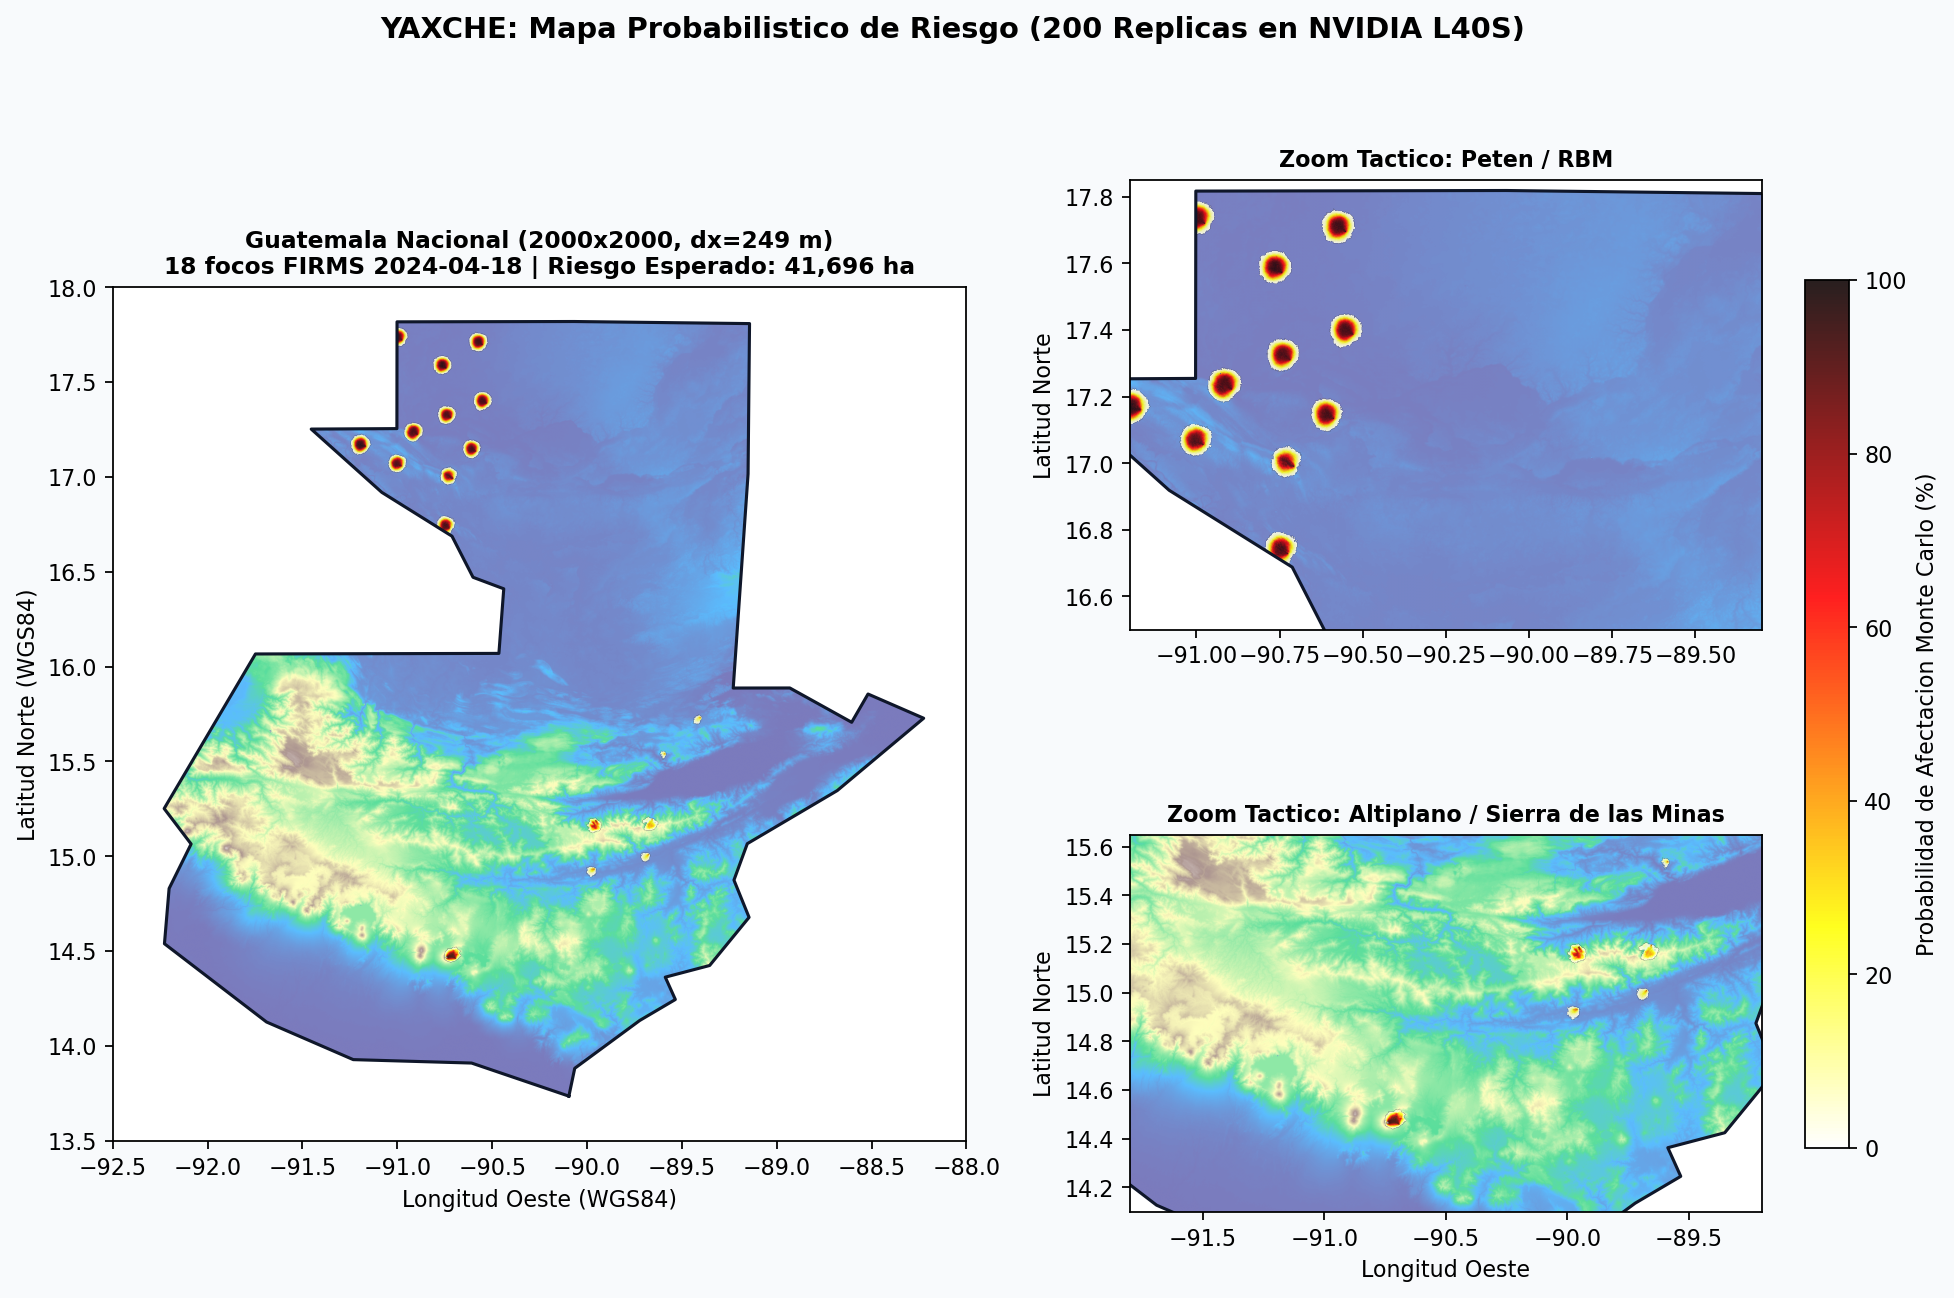
\includegraphics[width=\linewidth]{../results/riesgo_montecarlo.png}
\caption{Mapa probabilístico de riesgo Monte Carlo ($200$ réplicas en NVIDIA L40S) sobre malla real $2000\times 2000$ ($\Delta x = 249\text{ m}$) con acercamientos tácticos a Petén/RBM y Altiplano/Sierra de las Minas.}
\label{fig:mc}
\end{figure}

\subsection{Sensibilidad ante Meteorología en Vivo}

Para verificar la respuesta direccional del modelo ante datos meteorológicos actuales, se comparó el pronóstico a 48 horas partiendo de los mismos $18$ focos bajo el viento histórico de abril de 2024 ($3.60\text{ m/s}$, $91^\circ$ Este) frente al viento en vivo consultado en Open-Meteo en noviembre de 2026 ($1.82\text{ m/s}$, $315^\circ$ Noroeste). La Figura~\ref{fig:wind} muestra el giro de las plumas hacia el Sureste, modificando $10{,}259$ celdas y reduciendo el área proyectada de $43{,}334\text{ ha}$ a $27{,}581\text{ ha}$.

\begin{figure}[H]
\centering
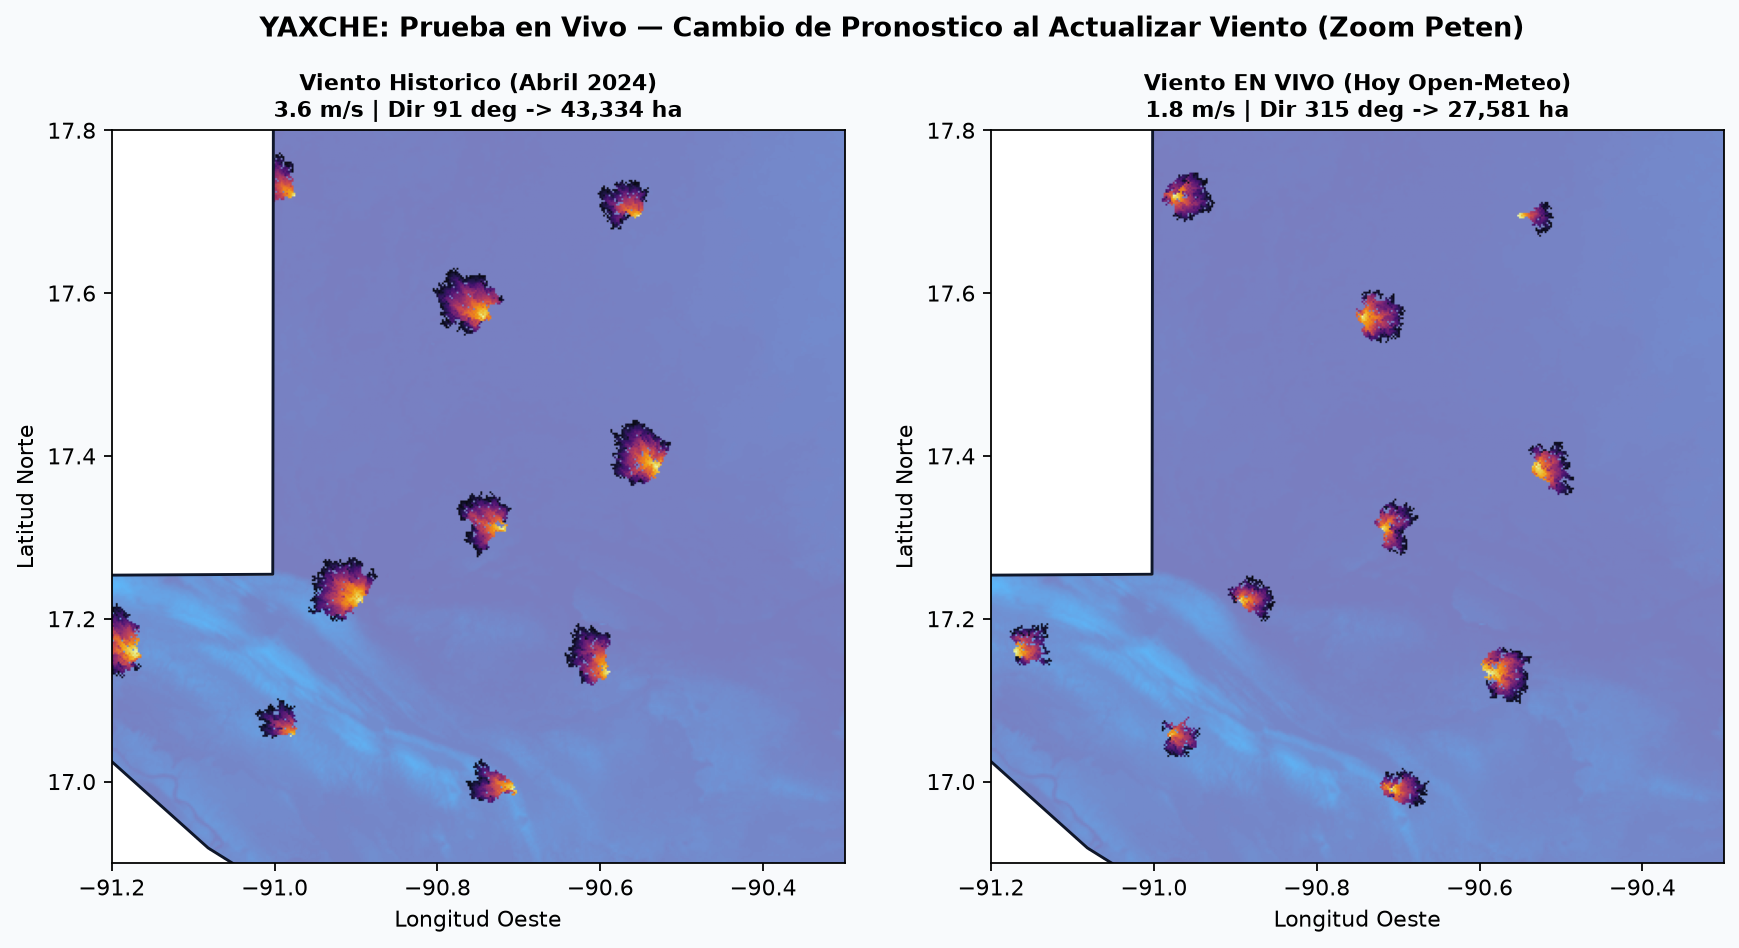
\includegraphics[width=\linewidth]{../results/comparativa_viento_vivo.png}
\caption{Comparativa de avance a 48 horas en el noroeste de Petén bajo viento histórico (abril 2024) y viento en vivo (noviembre 2026).}
\label{fig:wind}
\end{figure}

\section{Limitaciones y Trabajo Futuro}

Si bien YAXCHÉ demuestra aceleración GPU significativa y sensibilidad física coherente a escala nacional, para su transición hacia un sistema operativo institucional (CONRED, CONAP, INAB) se identifican cuatro líneas de trabajo futuro:

\begin{enumerate}
    \item \textbf{Calibración empírica (Backtesting):} ajustar los parámetros $p_{\text{base}}$, $c_s$ y $c_w$ mediante optimización en GPU comparando simulaciones a 48 horas contra perímetros históricos reales de incendios y detecciones consecutivas de NASA FIRMS ($t$ vs $t+48\text{ h}$) utilizando métricas espaciales como IoU y F1.
    \item \textbf{Mapas reales de cobertura y humedad vegetal:} sustituir la estimación topográfica de combustible por índices multiespectrales satelitales (NDVI/NBR de Sentinel-2 o MODIS).
    \item \textbf{Forzamiento meteorológico horario:} reemplazar el campo de viento estático por series horarias de viento, temperatura y humedad relativa.
    \item \textbf{Monte Carlo residente en VRAM:} mantener las mallas estáticas residentes en memoria de GPU entre réplicas para eliminar copias repetidas CPU--GPU y reducir el ensamble de $200$ réplicas por debajo de $2\text{ s}$.
\end{enumerate}

\section{Conclusiones}

Se presentó YAXCHÉ, un simulador físico de incendios forestales sobre Guatemala acelerado mediante Numba y CUDA. La paralelización masiva en GPU (NVIDIA L40S) con acceso coalescente a VRAM permitió alcanzar aceleraciones de hasta $1{,}021.7\times$ en cómputo de kernel respecto a CPU de 1 hilo en una malla real de $4\times 10^6$ celdas, habilitando ensambles Monte Carlo de $200$ réplicas en $11.11\text{ s}$ con determinismo bit-a-bit verificado.

\begin{thebibliography}{9}
\bibitem{rothermel1972}
R. C. Rothermel, ``A mathematical model for predicting fire spread in wildland fuels,'' USDA Forest Service, Intermountain Forest and Range Experiment Station, Res. Pap. INT-115, 1972.

\bibitem{finney1998}
M. A. Finney, ``FARSITE: Fire Area Simulator---Model development and evaluation,'' USDA Forest Service, Rocky Mountain Research Station, Res. Pap. RMRS-RP-4, 1998.

\bibitem{firms2024}
NASA FIRMS, ``Fire Information for Resource Management System (VIIRS 375m / MODIS),'' Earth Science Data and Information System (ESDIS), 2024--2026.

\bibitem{numba2015}
S. K. Lam, A. Pitrou, and S. Seibert, ``Numba: A LLVM-based Python JIT compiler,'' in \textit{Proc. Second Workshop on the LLVM Compiler Infrastructure in HPC}, 2015, pp. 1--6.
\end{thebibliography}

\end{document}

